% Created by tikzDevice version 0.12.3.1 on 2022-07-29 15:13:42
% !TEX encoding = UTF-8 Unicode
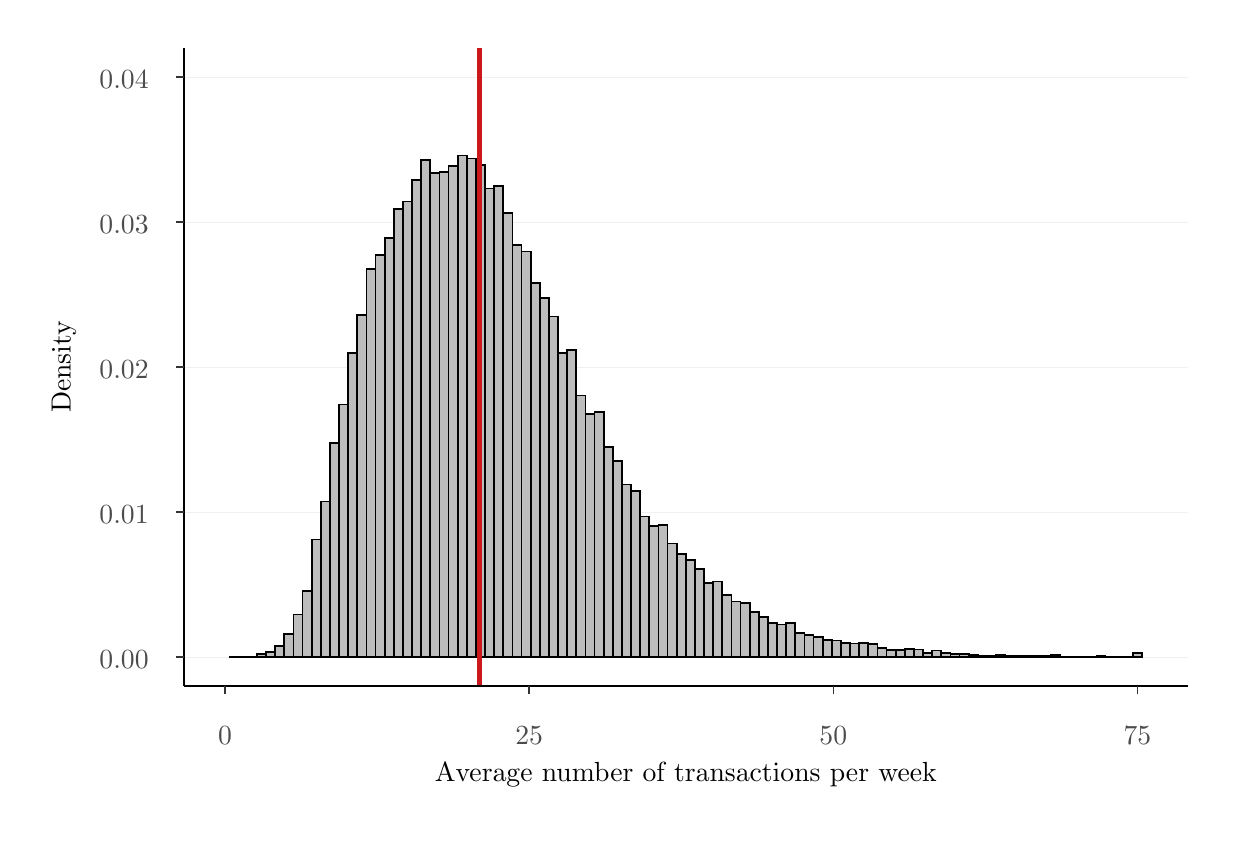
\begin{tikzpicture}[x=1pt,y=1pt]
\definecolor{fillColor}{RGB}{255,255,255}
\path[use as bounding box,fill=fillColor,fill opacity=0.00] (0,0) rectangle (433.62,289.08);
\begin{scope}
\path[clip] (  0.00,  0.00) rectangle (433.62,289.08);
\definecolor{drawColor}{RGB}{255,255,255}
\definecolor{fillColor}{RGB}{255,255,255}

\path[draw=drawColor,line width= 0.6pt,line join=round,line cap=round,fill=fillColor] ( -0.00,  0.00) rectangle (433.62,289.08);
\end{scope}
\begin{scope}
\path[clip] ( 56.47, 51.15) rectangle (419.17,281.85);
\definecolor{drawColor}{RGB}{255,255,255}

\path[draw=drawColor,line width= 0.3pt,line join=round] ( 56.47, 87.86) --
	(419.17, 87.86);

\path[draw=drawColor,line width= 0.3pt,line join=round] ( 56.47,140.29) --
	(419.17,140.29);

\path[draw=drawColor,line width= 0.3pt,line join=round] ( 56.47,192.72) --
	(419.17,192.72);

\path[draw=drawColor,line width= 0.3pt,line join=round] ( 56.47,245.15) --
	(419.17,245.15);

\path[draw=drawColor,line width= 0.3pt,line join=round] (126.26, 51.15) --
	(126.26,281.85);

\path[draw=drawColor,line width= 0.3pt,line join=round] (236.17, 51.15) --
	(236.17,281.85);

\path[draw=drawColor,line width= 0.3pt,line join=round] (346.08, 51.15) --
	(346.08,281.85);
\definecolor{drawColor}{gray}{0.94}

\path[draw=drawColor,line width= 0.1pt,line join=round] ( 56.47, 61.64) --
	(419.17, 61.64);

\path[draw=drawColor,line width= 0.1pt,line join=round] ( 56.47,114.07) --
	(419.17,114.07);

\path[draw=drawColor,line width= 0.1pt,line join=round] ( 56.47,166.50) --
	(419.17,166.50);

\path[draw=drawColor,line width= 0.1pt,line join=round] ( 56.47,218.93) --
	(419.17,218.93);

\path[draw=drawColor,line width= 0.1pt,line join=round] ( 56.47,271.37) --
	(419.17,271.37);
\definecolor{drawColor}{RGB}{0,0,0}
\definecolor{fillColor}{gray}{0.74}

\path[draw=drawColor,line width= 0.6pt,line cap=rect,fill=fillColor] ( 72.95, 61.64) rectangle ( 76.25, 61.71);

\path[draw=drawColor,line width= 0.6pt,line cap=rect,fill=fillColor] ( 76.25, 61.64) rectangle ( 79.55, 61.64);

\path[draw=drawColor,line width= 0.6pt,line cap=rect,fill=fillColor] ( 79.55, 61.64) rectangle ( 82.84, 61.79);

\path[draw=drawColor,line width= 0.6pt,line cap=rect,fill=fillColor] ( 82.84, 61.64) rectangle ( 86.14, 62.69);

\path[draw=drawColor,line width= 0.6pt,line cap=rect,fill=fillColor] ( 86.14, 61.64) rectangle ( 89.44, 63.43);

\path[draw=drawColor,line width= 0.6pt,line cap=rect,fill=fillColor] ( 89.44, 61.64) rectangle ( 92.74, 65.60);

\path[draw=drawColor,line width= 0.6pt,line cap=rect,fill=fillColor] ( 92.74, 61.64) rectangle ( 96.03, 69.94);

\path[draw=drawColor,line width= 0.6pt,line cap=rect,fill=fillColor] ( 96.03, 61.64) rectangle ( 99.33, 77.04);

\path[draw=drawColor,line width= 0.6pt,line cap=rect,fill=fillColor] ( 99.33, 61.64) rectangle (102.63, 85.56);

\path[draw=drawColor,line width= 0.6pt,line cap=rect,fill=fillColor] (102.63, 61.64) rectangle (105.92,104.17);

\path[draw=drawColor,line width= 0.6pt,line cap=rect,fill=fillColor] (105.92, 61.64) rectangle (109.22,117.92);

\path[draw=drawColor,line width= 0.6pt,line cap=rect,fill=fillColor] (109.22, 61.64) rectangle (112.52,138.92);

\path[draw=drawColor,line width= 0.6pt,line cap=rect,fill=fillColor] (112.52, 61.64) rectangle (115.82,152.97);

\path[draw=drawColor,line width= 0.6pt,line cap=rect,fill=fillColor] (115.82, 61.64) rectangle (119.11,171.51);

\path[draw=drawColor,line width= 0.6pt,line cap=rect,fill=fillColor] (119.11, 61.64) rectangle (122.41,185.19);

\path[draw=drawColor,line width= 0.6pt,line cap=rect,fill=fillColor] (122.41, 61.64) rectangle (125.71,201.85);

\path[draw=drawColor,line width= 0.6pt,line cap=rect,fill=fillColor] (125.71, 61.64) rectangle (129.01,206.94);

\path[draw=drawColor,line width= 0.6pt,line cap=rect,fill=fillColor] (129.01, 61.64) rectangle (132.30,213.14);

\path[draw=drawColor,line width= 0.6pt,line cap=rect,fill=fillColor] (132.30, 61.64) rectangle (135.60,223.53);

\path[draw=drawColor,line width= 0.6pt,line cap=rect,fill=fillColor] (135.60, 61.64) rectangle (138.90,226.22);

\path[draw=drawColor,line width= 0.6pt,line cap=rect,fill=fillColor] (138.90, 61.64) rectangle (142.19,234.07);

\path[draw=drawColor,line width= 0.6pt,line cap=rect,fill=fillColor] (142.19, 61.64) rectangle (145.49,241.17);

\path[draw=drawColor,line width= 0.6pt,line cap=rect,fill=fillColor] (145.49, 61.64) rectangle (148.79,236.46);

\path[draw=drawColor,line width= 0.6pt,line cap=rect,fill=fillColor] (148.79, 61.64) rectangle (152.09,236.98);

\path[draw=drawColor,line width= 0.6pt,line cap=rect,fill=fillColor] (152.09, 61.64) rectangle (155.38,239.08);

\path[draw=drawColor,line width= 0.6pt,line cap=rect,fill=fillColor] (155.38, 61.64) rectangle (158.68,242.89);

\path[draw=drawColor,line width= 0.6pt,line cap=rect,fill=fillColor] (158.68, 61.64) rectangle (161.98,241.77);

\path[draw=drawColor,line width= 0.6pt,line cap=rect,fill=fillColor] (161.98, 61.64) rectangle (165.28,239.45);

\path[draw=drawColor,line width= 0.6pt,line cap=rect,fill=fillColor] (165.28, 61.64) rectangle (168.57,231.00);

\path[draw=drawColor,line width= 0.6pt,line cap=rect,fill=fillColor] (168.57, 61.64) rectangle (171.87,231.98);

\path[draw=drawColor,line width= 0.6pt,line cap=rect,fill=fillColor] (171.87, 61.64) rectangle (175.17,222.03);

\path[draw=drawColor,line width= 0.6pt,line cap=rect,fill=fillColor] (175.17, 61.64) rectangle (178.46,210.45);

\path[draw=drawColor,line width= 0.6pt,line cap=rect,fill=fillColor] (178.46, 61.64) rectangle (181.76,208.21);

\path[draw=drawColor,line width= 0.6pt,line cap=rect,fill=fillColor] (181.76, 61.64) rectangle (185.06,196.85);

\path[draw=drawColor,line width= 0.6pt,line cap=rect,fill=fillColor] (185.06, 61.64) rectangle (188.36,191.39);

\path[draw=drawColor,line width= 0.6pt,line cap=rect,fill=fillColor] (188.36, 61.64) rectangle (191.65,184.74);

\path[draw=drawColor,line width= 0.6pt,line cap=rect,fill=fillColor] (191.65, 61.64) rectangle (194.95,171.58);

\path[draw=drawColor,line width= 0.6pt,line cap=rect,fill=fillColor] (194.95, 61.64) rectangle (198.25,172.56);

\path[draw=drawColor,line width= 0.6pt,line cap=rect,fill=fillColor] (198.25, 61.64) rectangle (201.55,156.19);

\path[draw=drawColor,line width= 0.6pt,line cap=rect,fill=fillColor] (201.55, 61.64) rectangle (204.84,149.39);

\path[draw=drawColor,line width= 0.6pt,line cap=rect,fill=fillColor] (204.84, 61.64) rectangle (208.14,150.21);

\path[draw=drawColor,line width= 0.6pt,line cap=rect,fill=fillColor] (208.14, 61.64) rectangle (211.44,137.65);

\path[draw=drawColor,line width= 0.6pt,line cap=rect,fill=fillColor] (211.44, 61.64) rectangle (214.73,132.42);

\path[draw=drawColor,line width= 0.6pt,line cap=rect,fill=fillColor] (214.73, 61.64) rectangle (218.03,123.97);

\path[draw=drawColor,line width= 0.6pt,line cap=rect,fill=fillColor] (218.03, 61.64) rectangle (221.33,121.73);

\path[draw=drawColor,line width= 0.6pt,line cap=rect,fill=fillColor] (221.33, 61.64) rectangle (224.63,112.39);

\path[draw=drawColor,line width= 0.6pt,line cap=rect,fill=fillColor] (224.63, 61.64) rectangle (227.92,109.10);

\path[draw=drawColor,line width= 0.6pt,line cap=rect,fill=fillColor] (227.92, 61.64) rectangle (231.22,109.47);

\path[draw=drawColor,line width= 0.6pt,line cap=rect,fill=fillColor] (231.22, 61.64) rectangle (234.52,102.67);

\path[draw=drawColor,line width= 0.6pt,line cap=rect,fill=fillColor] (234.52, 61.64) rectangle (237.82, 98.79);

\path[draw=drawColor,line width= 0.6pt,line cap=rect,fill=fillColor] (237.82, 61.64) rectangle (241.11, 96.84);

\path[draw=drawColor,line width= 0.6pt,line cap=rect,fill=fillColor] (241.11, 61.64) rectangle (244.41, 93.40);

\path[draw=drawColor,line width= 0.6pt,line cap=rect,fill=fillColor] (244.41, 61.64) rectangle (247.71, 88.47);

\path[draw=drawColor,line width= 0.6pt,line cap=rect,fill=fillColor] (247.71, 61.64) rectangle (251.00, 88.92);

\path[draw=drawColor,line width= 0.6pt,line cap=rect,fill=fillColor] (251.00, 61.64) rectangle (254.30, 83.99);

\path[draw=drawColor,line width= 0.6pt,line cap=rect,fill=fillColor] (254.30, 61.64) rectangle (257.60, 81.67);

\path[draw=drawColor,line width= 0.6pt,line cap=rect,fill=fillColor] (257.60, 61.64) rectangle (260.90, 81.15);

\path[draw=drawColor,line width= 0.6pt,line cap=rect,fill=fillColor] (260.90, 61.64) rectangle (264.19, 77.93);

\path[draw=drawColor,line width= 0.6pt,line cap=rect,fill=fillColor] (264.19, 61.64) rectangle (267.49, 76.06);

\path[draw=drawColor,line width= 0.6pt,line cap=rect,fill=fillColor] (267.49, 61.64) rectangle (270.79, 74.05);

\path[draw=drawColor,line width= 0.6pt,line cap=rect,fill=fillColor] (270.79, 61.64) rectangle (274.09, 73.37);

\path[draw=drawColor,line width= 0.6pt,line cap=rect,fill=fillColor] (274.09, 61.64) rectangle (277.38, 73.90);

\path[draw=drawColor,line width= 0.6pt,line cap=rect,fill=fillColor] (277.38, 61.64) rectangle (280.68, 70.24);

\path[draw=drawColor,line width= 0.6pt,line cap=rect,fill=fillColor] (280.68, 61.64) rectangle (283.98, 69.71);

\path[draw=drawColor,line width= 0.6pt,line cap=rect,fill=fillColor] (283.98, 61.64) rectangle (287.27, 68.89);

\path[draw=drawColor,line width= 0.6pt,line cap=rect,fill=fillColor] (287.27, 61.64) rectangle (290.57, 67.92);

\path[draw=drawColor,line width= 0.6pt,line cap=rect,fill=fillColor] (290.57, 61.64) rectangle (293.87, 67.69);

\path[draw=drawColor,line width= 0.6pt,line cap=rect,fill=fillColor] (293.87, 61.64) rectangle (297.17, 66.80);

\path[draw=drawColor,line width= 0.6pt,line cap=rect,fill=fillColor] (297.17, 61.64) rectangle (300.46, 66.57);

\path[draw=drawColor,line width= 0.6pt,line cap=rect,fill=fillColor] (300.46, 61.64) rectangle (303.76, 66.65);

\path[draw=drawColor,line width= 0.6pt,line cap=rect,fill=fillColor] (303.76, 61.64) rectangle (307.06, 66.42);

\path[draw=drawColor,line width= 0.6pt,line cap=rect,fill=fillColor] (307.06, 61.64) rectangle (310.36, 64.93);

\path[draw=drawColor,line width= 0.6pt,line cap=rect,fill=fillColor] (310.36, 61.64) rectangle (313.65, 64.11);

\path[draw=drawColor,line width= 0.6pt,line cap=rect,fill=fillColor] (313.65, 61.64) rectangle (316.95, 64.26);

\path[draw=drawColor,line width= 0.6pt,line cap=rect,fill=fillColor] (316.95, 61.64) rectangle (320.25, 64.55);

\path[draw=drawColor,line width= 0.6pt,line cap=rect,fill=fillColor] (320.25, 61.64) rectangle (323.55, 64.33);

\path[draw=drawColor,line width= 0.6pt,line cap=rect,fill=fillColor] (323.55, 61.64) rectangle (326.84, 63.21);

\path[draw=drawColor,line width= 0.6pt,line cap=rect,fill=fillColor] (326.84, 61.64) rectangle (330.14, 64.03);

\path[draw=drawColor,line width= 0.6pt,line cap=rect,fill=fillColor] (330.14, 61.64) rectangle (333.44, 63.21);

\path[draw=drawColor,line width= 0.6pt,line cap=rect,fill=fillColor] (333.44, 61.64) rectangle (336.73, 62.76);

\path[draw=drawColor,line width= 0.6pt,line cap=rect,fill=fillColor] (336.73, 61.64) rectangle (340.03, 62.69);

\path[draw=drawColor,line width= 0.6pt,line cap=rect,fill=fillColor] (340.03, 61.64) rectangle (343.33, 62.39);

\path[draw=drawColor,line width= 0.6pt,line cap=rect,fill=fillColor] (343.33, 61.64) rectangle (346.63, 62.16);

\path[draw=drawColor,line width= 0.6pt,line cap=rect,fill=fillColor] (346.63, 61.64) rectangle (349.92, 62.09);

\path[draw=drawColor,line width= 0.6pt,line cap=rect,fill=fillColor] (349.92, 61.64) rectangle (353.22, 62.46);

\path[draw=drawColor,line width= 0.6pt,line cap=rect,fill=fillColor] (353.22, 61.64) rectangle (356.52, 62.24);

\path[draw=drawColor,line width= 0.6pt,line cap=rect,fill=fillColor] (356.52, 61.64) rectangle (359.82, 62.24);

\path[draw=drawColor,line width= 0.6pt,line cap=rect,fill=fillColor] (359.82, 61.64) rectangle (363.11, 62.16);

\path[draw=drawColor,line width= 0.6pt,line cap=rect,fill=fillColor] (363.11, 61.64) rectangle (366.41, 61.94);

\path[draw=drawColor,line width= 0.6pt,line cap=rect,fill=fillColor] (366.41, 61.64) rectangle (369.71, 62.09);

\path[draw=drawColor,line width= 0.6pt,line cap=rect,fill=fillColor] (369.71, 61.64) rectangle (373.00, 62.46);

\path[draw=drawColor,line width= 0.6pt,line cap=rect,fill=fillColor] (373.00, 61.64) rectangle (376.30, 61.79);

\path[draw=drawColor,line width= 0.6pt,line cap=rect,fill=fillColor] (376.30, 61.64) rectangle (379.60, 61.86);

\path[draw=drawColor,line width= 0.6pt,line cap=rect,fill=fillColor] (379.60, 61.64) rectangle (382.90, 61.86);

\path[draw=drawColor,line width= 0.6pt,line cap=rect,fill=fillColor] (382.90, 61.64) rectangle (386.19, 61.86);

\path[draw=drawColor,line width= 0.6pt,line cap=rect,fill=fillColor] (386.19, 61.64) rectangle (389.49, 61.94);

\path[draw=drawColor,line width= 0.6pt,line cap=rect,fill=fillColor] (389.49, 61.64) rectangle (392.79, 61.79);

\path[draw=drawColor,line width= 0.6pt,line cap=rect,fill=fillColor] (392.79, 61.64) rectangle (396.09, 61.86);

\path[draw=drawColor,line width= 0.6pt,line cap=rect,fill=fillColor] (396.09, 61.64) rectangle (399.38, 61.79);

\path[draw=drawColor,line width= 0.6pt,line cap=rect,fill=fillColor] (399.38, 61.64) rectangle (402.68, 63.06);
\definecolor{drawColor}{RGB}{203,24,29}

\path[draw=drawColor,line width= 1.7pt,line join=round] (163.20, 51.15) -- (163.20,281.85);
\end{scope}
\begin{scope}
\path[clip] (  0.00,  0.00) rectangle (433.62,289.08);
\definecolor{drawColor}{RGB}{0,0,0}

\path[draw=drawColor,line width= 0.6pt,line join=round] ( 56.47, 51.15) --
	( 56.47,281.85);
\end{scope}
\begin{scope}
\path[clip] (  0.00,  0.00) rectangle (433.62,289.08);
\definecolor{drawColor}{gray}{0.30}

\node[text=drawColor,anchor=base east,inner sep=0pt, outer sep=0pt, scale=  1.00] at ( 43.72, 57.51) {0.00};

\node[text=drawColor,anchor=base east,inner sep=0pt, outer sep=0pt, scale=  1.00] at ( 43.72,109.94) {0.01};

\node[text=drawColor,anchor=base east,inner sep=0pt, outer sep=0pt, scale=  1.00] at ( 43.72,162.37) {0.02};

\node[text=drawColor,anchor=base east,inner sep=0pt, outer sep=0pt, scale=  1.00] at ( 43.72,214.80) {0.03};

\node[text=drawColor,anchor=base east,inner sep=0pt, outer sep=0pt, scale=  1.00] at ( 43.72,267.23) {0.04};
\end{scope}
\begin{scope}
\path[clip] (  0.00,  0.00) rectangle (433.62,289.08);
\definecolor{drawColor}{gray}{0.20}

\path[draw=drawColor,line width= 0.6pt,line join=round] ( 53.72, 61.64) --
	( 56.47, 61.64);

\path[draw=drawColor,line width= 0.6pt,line join=round] ( 53.72,114.07) --
	( 56.47,114.07);

\path[draw=drawColor,line width= 0.6pt,line join=round] ( 53.72,166.50) --
	( 56.47,166.50);

\path[draw=drawColor,line width= 0.6pt,line join=round] ( 53.72,218.93) --
	( 56.47,218.93);

\path[draw=drawColor,line width= 0.6pt,line join=round] ( 53.72,271.37) --
	( 56.47,271.37);
\end{scope}
\begin{scope}
\path[clip] (  0.00,  0.00) rectangle (433.62,289.08);
\definecolor{drawColor}{RGB}{0,0,0}

\path[draw=drawColor,line width= 0.6pt,line join=round] ( 56.47, 51.15) --
	(419.17, 51.15);
\end{scope}
\begin{scope}
\path[clip] (  0.00,  0.00) rectangle (433.62,289.08);
\definecolor{drawColor}{gray}{0.20}

\path[draw=drawColor,line width= 0.6pt,line join=round] ( 71.30, 48.40) --
	( 71.30, 51.15);

\path[draw=drawColor,line width= 0.6pt,line join=round] (181.21, 48.40) --
	(181.21, 51.15);

\path[draw=drawColor,line width= 0.6pt,line join=round] (291.12, 48.40) --
	(291.12, 51.15);

\path[draw=drawColor,line width= 0.6pt,line join=round] (401.03, 48.40) --
	(401.03, 51.15);
\end{scope}
\begin{scope}
\path[clip] (  0.00,  0.00) rectangle (433.62,289.08);
\definecolor{drawColor}{gray}{0.30}

\node[text=drawColor,anchor=base,inner sep=0pt, outer sep=0pt, scale=  1.00] at ( 71.30, 30.14) {0};

\node[text=drawColor,anchor=base,inner sep=0pt, outer sep=0pt, scale=  1.00] at (181.21, 30.14) {25};

\node[text=drawColor,anchor=base,inner sep=0pt, outer sep=0pt, scale=  1.00] at (291.12, 30.14) {50};

\node[text=drawColor,anchor=base,inner sep=0pt, outer sep=0pt, scale=  1.00] at (401.03, 30.14) {75};
\end{scope}
\begin{scope}
\path[clip] (  0.00,  0.00) rectangle (433.62,289.08);
\definecolor{drawColor}{RGB}{0,0,0}

\node[text=drawColor,anchor=base,inner sep=0pt, outer sep=0pt, scale=  1.00] at (237.82, 16.79) {Average number of transactions per week};
\end{scope}
\begin{scope}
\path[clip] (  0.00,  0.00) rectangle (433.62,289.08);
\definecolor{drawColor}{RGB}{0,0,0}

\node[text=drawColor,rotate= 90.00,anchor=base,inner sep=0pt, outer sep=0pt, scale=  1.00] at ( 15.49,166.50) {Density};
\end{scope}
\end{tikzpicture}
